\subsubsection{Model View Presenter}
The structure imposed by the chosen multi-tier architecture suggests the use of the \textbf{MVP} (Model-View-Presenter) architectural pattern.\\
Here are briefly presented the concept behind the \textbf{MVP} architecture, with respect to the component used in the service.
\begin{itemize}
    \item \textbf{Model}: Handles the communication with the database.
    \item \textbf{View}: Handles the information displayed to the generic user, therefore being, in this situation, completely passive.
    \item \textbf{Presenter}: Serves as a middleware manipulating data exposed via queries by the \textbf{Model} in response to events dispatched by a generic user (e.g Login, request for subscription etc)
\end{itemize}
\begin{center}
    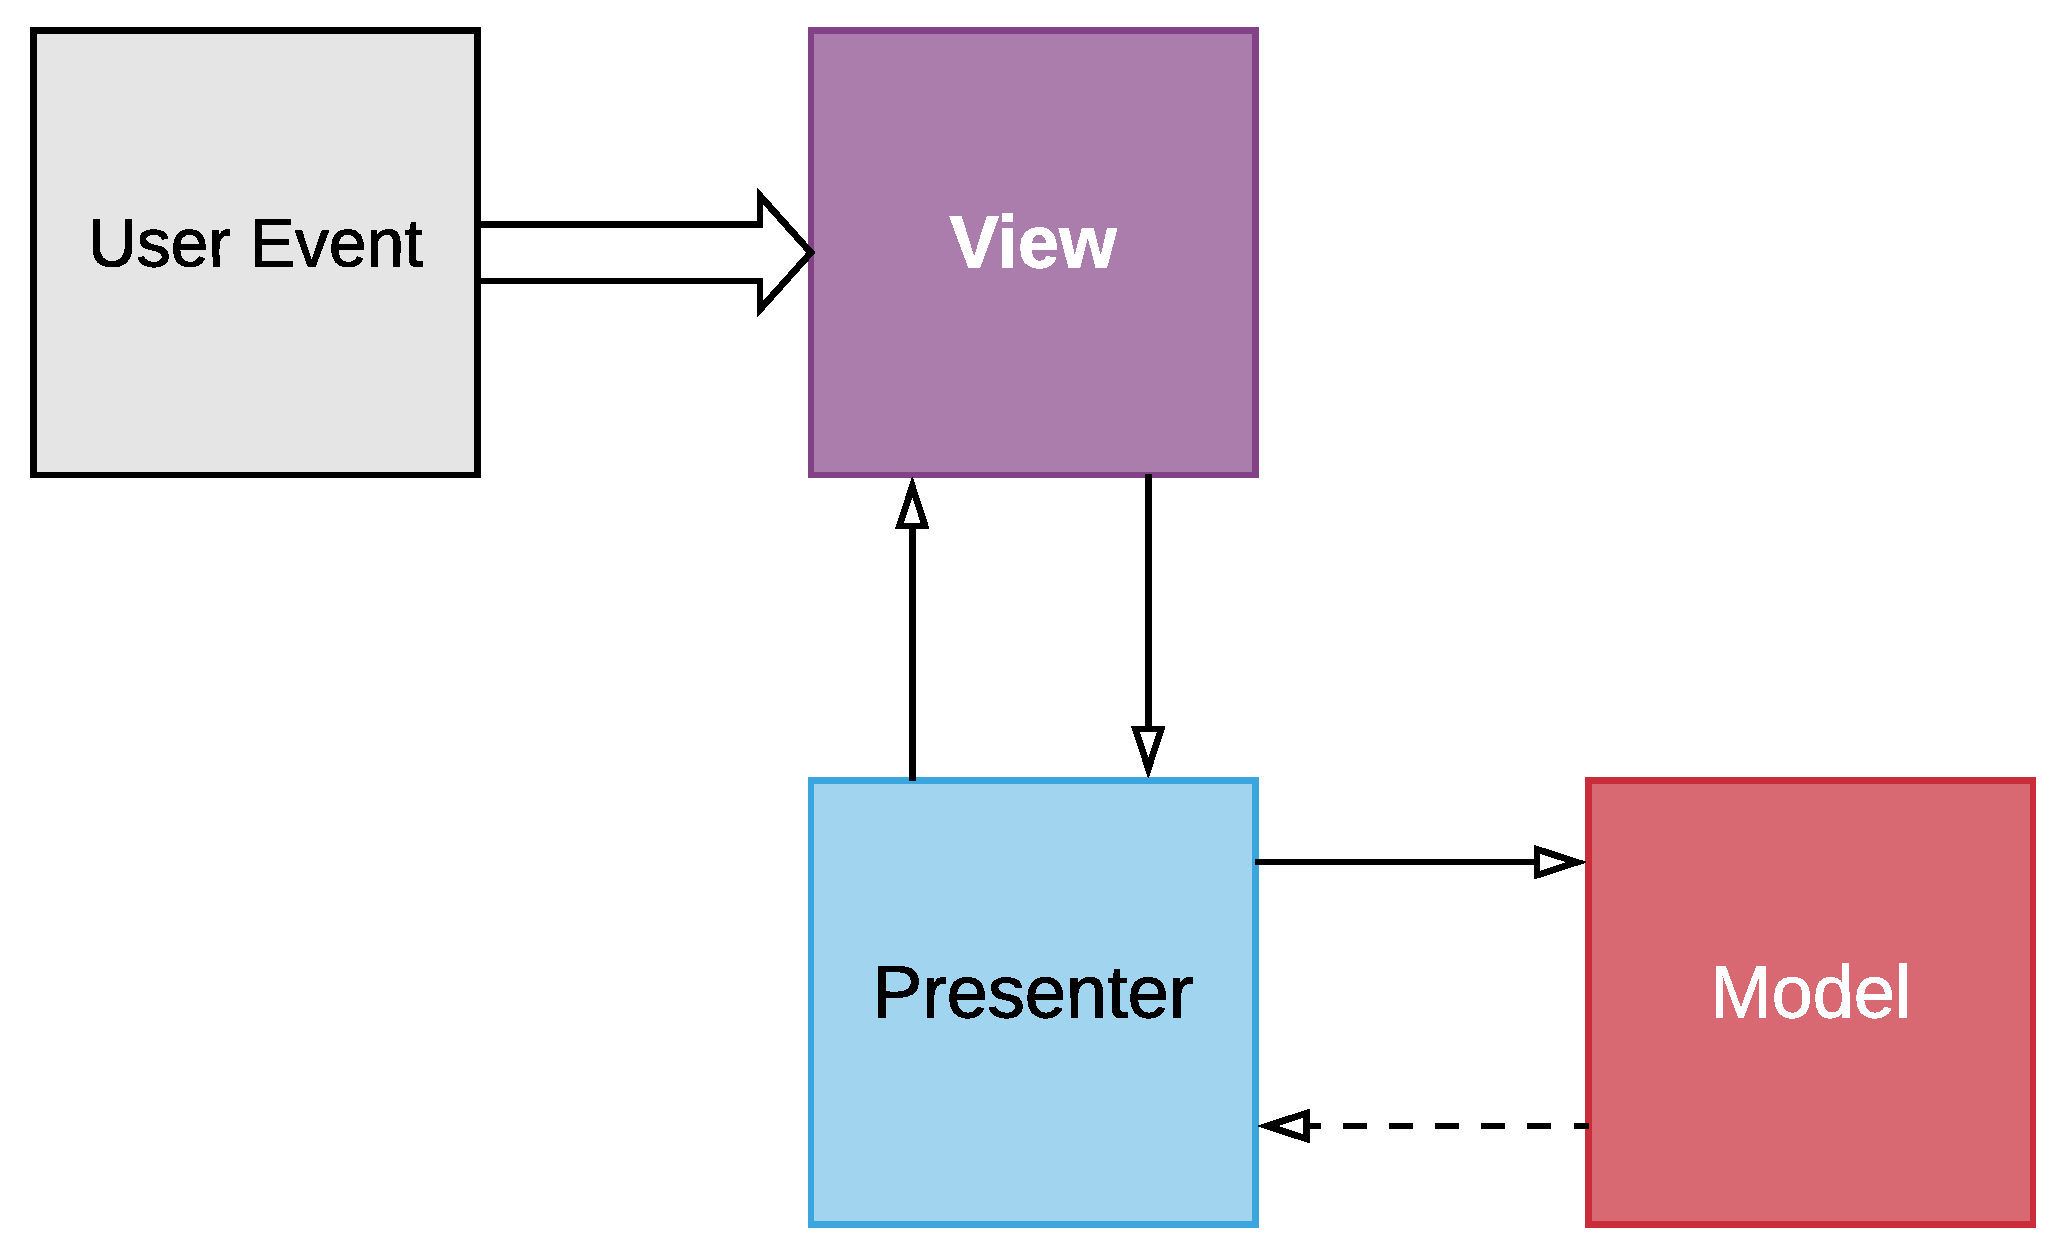
\includegraphics[width=0.5\textwidth]{assets/MVP.pdf}
\end{center}

\subsubsection{Stateless}
In order to easily serve more or less users according to the demand of the service it has been opted for a stateless \textit{Business Logic Tier}. This allows the service to be scaled when needed, therefore saving resources when requests are low. 
